\section{CSGCN-IS}\label{sec:csgcn_is}
This section describes the first of our two proposed models, Context and Side-information GCN with Item-Splitting (CSGCN-IS), which is a GCN that incorporates side-information in the graph, and considers context as an embedding.

\subsection{Model intuition}\label{subsec:csgcn_is_intuition}
Before diving into the details of how CSGCN-IS is modeled, let us examine the intuition behind it.
The goal is to construct a model that can generate a top-$k$ list of recommendations for a user, both in a context-aware recommendation setting, using the given context that the user is in, and in a regular non-context-aware setting.
To do this, we start out by expressing the available information in a graph.
This mainly includes interactions between users and items.
However, since most RS datasets are sparse, we want to see if we can alleviate this problem by further connecting user and item nodes, to improve the collaborative signals in the model.
To do this, we utilize the fact that most datasets include some amount of additional information about users and items.
This additional information can be used to further connect users and items by adding it as nodes in the graph.\\
Besides side-information, we need to reason about how to express context in the model.
After experimenting with various ways to express this, we came to the realization that context can be simplified to be a modifier to an item, which signifies whether the items are popular in a given context or not.
For example, we may learn that indoor activities are generally more popular on a rainy day.
This can be learned by the model through sampling user interactions in various contexts from ground truth.
For the user and context sampled, we see that they interacted with a given item, which should lead to an increase in the context score for this item-context combination.
At the same time, we find a negative sample for the same user and context and decrease the item-context score for the item that is not interacted with in this context, to signify that, for example, going for a hike is not a popular choice on a rainy day.\\
With this intuition, we will now detail how this is implemented in the CSGCN model.

\subsection{Model architecture}\label{subsec:csgcn_is_model_architecture}
While traditional GCN models make use of three main ideas: Feature propagation of neighbor nodes, linear transformation and nonlinear activation, several well-cited papers \cite{SimplifyingGCN,LightGCN,HeteGCN} suggest that this is largely caused by the history of GCNs.
Wu et al. presents the idea that while most machine learning algorithms followed a clear path from an initial simple model to a more complex model through the needs of more expressivity, this was not the case of GCNs.
Instead, they were proposed in the recent years of neural networks where deep learning had gained high popularity, and as such GCNs were built directly on top of a complex model.
To investigate whether this was useful, they present SGCN, a simplified version of GCNs that could have preceeded GCNs if the traditional path had been taken.
This led them to remove the linear transformation and nonlinear activation, to reach a simplified linear model.
Interestingly, they proved that not only does this not degrade performance of the models, it generally matches or improves both in terms of performance and speed \cite{SimplifyingGCN}.\\
This signifies that the expressive power of GCNs originates primarily from the propagations done in the convolution layers, rather than the nonlinear feature extractions we know from traditional GCNs \cite{SimplifyingGCN}.
Based on these considerations, the CSGCN models are based on these observations made in the SGCN \cite{SimplifyingGCN} and the LightGCN model \cite{LightGCN}, which has applied these considerations and proven that it outperforms regular GCNs that employ a traditional GCN model with all three components \cite{LightGCN}.



%\begin{figure}[hbt!]
	%\hspace*{-0.1cm}
%	\centering
%	\small	
%	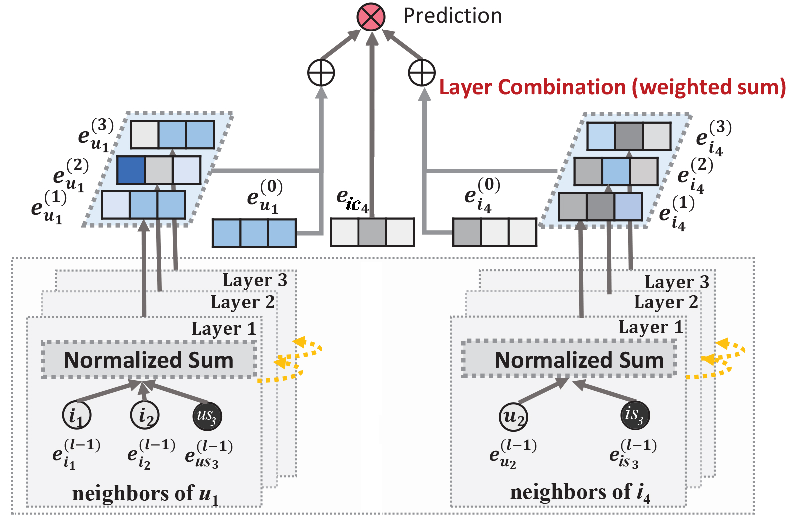
\includegraphics[width=0.48\textwidth]{figures/CSGCN.pdf}\vspace{-5pt}
%	\caption{An illustration of CSGCN-IS model architecture. User and item neighbors are illustrated as bright nodes, and side-information as dark nodes. In the layer combination, we sum over the embeddings at each layer to obtain the final representations.}\vspace{-10pt}
%	\label{fig:csgcn_is_model}
%\end{figure}
The model itself is very similar to LightGCN.
It is, however, important to note that the neighboring nodes for users now include side-information for users and not only items, which can be seen in each of the layers now receiving a normalized sum of both items and user side-information, rather than just the normalized sum of items.
The same goes for the neighbors of items.
\\
There are a number of graph convolution layers that update the representation of each central node with information about their neighbor nodes.
The representation at layer $l+1$ is calculated by taking the normalized sum of the representations of neighbor nodes at layer $l$. 
As mentioned, neighbor nodes for user are item nodes and user side-information nodes, and for items the neighbors are user nodes and item side-information nodes, which can be seen on \Cref{fig:quadripartite-graph}.
For each additional layer, information is passed from nodes that are further away from a central node, illustrated on \Cref{fig:aggregation-for-layers}
After $n$ layers the representations at each of the layers are aggregated into a final representation.
From these final representations, a score prediction can be calculated between an item, user and a context which is further described in \Cref{subsec:csgcn_is_score_prediction}.



\begin{figure}[h]
\centering



\tikzset{every picture/.style={line width=0.75pt}} %set default line width to 0.75pt        

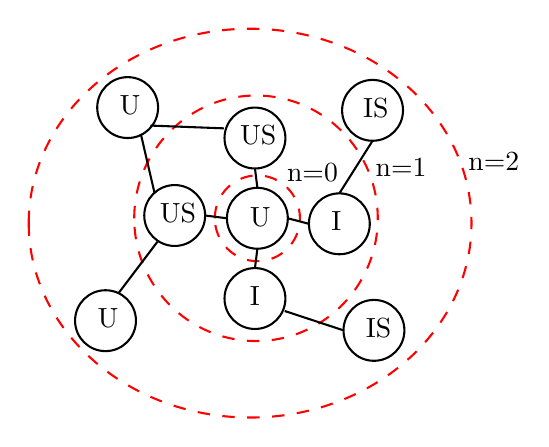
\begin{tikzpicture}[x=0.5pt,y=0.5pt,yscale=-1,xscale=1]
%uncomment if require: \path (0,300); %set diagram left start at 0, and has height of 300

%Flowchart: Connector [id:dp27406580802635316] 
\draw   (290.75,139) .. controls (290.75,126.85) and (300.6,117) .. (312.75,117) .. controls (324.9,117) and (334.75,126.85) .. (334.75,139) .. controls (334.75,151.15) and (324.9,161) .. (312.75,161) .. controls (300.6,161) and (290.75,151.15) .. (290.75,139) -- cycle ;
%Flowchart: Connector [id:dp597318920352127] 
\draw   (289,81) .. controls (289,68.85) and (298.85,59) .. (311,59) .. controls (323.15,59) and (333,68.85) .. (333,81) .. controls (333,93.15) and (323.15,103) .. (311,103) .. controls (298.85,103) and (289,93.15) .. (289,81) -- cycle ;
%Flowchart: Connector [id:dp057928841134587516] 
\draw   (350,143) .. controls (350,130.85) and (359.85,121) .. (372,121) .. controls (384.15,121) and (394,130.85) .. (394,143) .. controls (394,155.15) and (384.15,165) .. (372,165) .. controls (359.85,165) and (350,155.15) .. (350,143) -- cycle ;
%Flowchart: Connector [id:dp11200641374570286] 
\draw   (289,197) .. controls (289,184.85) and (298.85,175) .. (311,175) .. controls (323.15,175) and (333,184.85) .. (333,197) .. controls (333,209.15) and (323.15,219) .. (311,219) .. controls (298.85,219) and (289,209.15) .. (289,197) -- cycle ;
%Flowchart: Connector [id:dp5153973147602738] 
\draw   (231,137) .. controls (231,124.85) and (240.85,115) .. (253,115) .. controls (265.15,115) and (275,124.85) .. (275,137) .. controls (275,149.15) and (265.15,159) .. (253,159) .. controls (240.85,159) and (231,149.15) .. (231,137) -- cycle ;
%Flowchart: Connector [id:dp6230129861696904] 
\draw   (197,59) .. controls (197,46.85) and (206.85,37) .. (219,37) .. controls (231.15,37) and (241,46.85) .. (241,59) .. controls (241,71.15) and (231.15,81) .. (219,81) .. controls (206.85,81) and (197,71.15) .. (197,59) -- cycle ;
%Flowchart: Connector [id:dp11627558541491778] 
\draw   (181,213) .. controls (181,200.85) and (190.85,191) .. (203,191) .. controls (215.15,191) and (225,200.85) .. (225,213) .. controls (225,225.15) and (215.15,235) .. (203,235) .. controls (190.85,235) and (181,225.15) .. (181,213) -- cycle ;
%Flowchart: Connector [id:dp012014051199046416] 
\draw   (374,61) .. controls (374,48.85) and (383.85,39) .. (396,39) .. controls (408.15,39) and (418,48.85) .. (418,61) .. controls (418,73.15) and (408.15,83) .. (396,83) .. controls (383.85,83) and (374,73.15) .. (374,61) -- cycle ;
%Flowchart: Connector [id:dp025105219979997373] 
\draw   (375,220) .. controls (375,207.85) and (384.85,198) .. (397,198) .. controls (409.15,198) and (419,207.85) .. (419,220) .. controls (419,232.15) and (409.15,242) .. (397,242) .. controls (384.85,242) and (375,232.15) .. (375,220) -- cycle ;
%Flowchart: Connector [id:dp28306483017107376] 
\draw  [color={rgb, 255:red, 255; green, 0; blue, 0 }  ,draw opacity=1 ][dash pattern={on 4.5pt off 4.5pt}] (282,139) .. controls (282,121.88) and (295.77,108) .. (312.75,108) .. controls (329.73,108) and (343.5,121.88) .. (343.5,139) .. controls (343.5,156.12) and (329.73,170) .. (312.75,170) .. controls (295.77,170) and (282,156.12) .. (282,139) -- cycle ;
%Flowchart: Connector [id:dp22791557868185153] 
\draw  [color={rgb, 255:red, 255; green, 0; blue, 0 }  ,draw opacity=1 ][dash pattern={on 4.5pt off 4.5pt}] (223.75,139) .. controls (223.75,90) and (263.15,50.28) .. (311.75,50.28) .. controls (360.35,50.28) and (399.75,90) .. (399.75,139) .. controls (399.75,188) and (360.35,227.72) .. (311.75,227.72) .. controls (263.15,227.72) and (223.75,188) .. (223.75,139) -- cycle ;
%Flowchart: Connector [id:dp946514520124221] 
\draw  [color={rgb, 255:red, 255; green, 0; blue, 0 }  ,draw opacity=1 ][dash pattern={on 4.5pt off 4.5pt}] (147.5,142.5) .. controls (147.5,64.9) and (219.13,2) .. (307.5,2) .. controls (395.87,2) and (467.5,64.9) .. (467.5,142.5) .. controls (467.5,220.1) and (395.87,283) .. (307.5,283) .. controls (219.13,283) and (147.5,220.1) .. (147.5,142.5) -- cycle ;
%Straight Lines [id:da566741285857424] 
\draw    (235.5,72) -- (288.5,74) ;
%Straight Lines [id:da31194843739323463] 
\draw    (228.5,78) -- (238.5,121) ;
%Straight Lines [id:da32353885946741523] 
\draw    (240.5,156) -- (212.5,193) ;
%Straight Lines [id:da5053069271391968] 
\draw    (311,103) -- (312.75,117) ;
%Straight Lines [id:da723620476456976] 
\draw    (290.75,139) -- (275,137) ;
%Straight Lines [id:da14267027138513144] 
\draw    (312.75,161) -- (311,175) ;
%Straight Lines [id:da6090096595211273] 
\draw    (334.75,139) -- (350,143) ;
%Straight Lines [id:da11771537978983193] 
\draw    (396,83) -- (372,121) ;
%Straight Lines [id:da45445879447578685] 
\draw    (332.5,206) -- (375,220) ;

% Text Node
\draw (305,129) node [anchor=north west][inner sep=0.75pt]   [align=left] {U};
% Text Node
\draw (298,70) node [anchor=north west][inner sep=0.75pt]   [align=left] {US};
% Text Node
\draw (364,132) node [anchor=north west][inner sep=0.75pt]   [align=left] {I};
% Text Node
\draw (305,186) node [anchor=north west][inner sep=0.75pt]   [align=left] {I};
% Text Node
\draw (240,126) node [anchor=north west][inner sep=0.75pt]   [align=left] {US};
% Text Node
\draw (211,48) node [anchor=north west][inner sep=0.75pt]   [align=left] {U};
% Text Node
\draw (195,202) node [anchor=north west][inner sep=0.75pt]   [align=left] {U};
% Text Node
\draw (387,50) node [anchor=north west][inner sep=0.75pt]   [align=left] {IS};
% Text Node
\draw (389,209) node [anchor=north west][inner sep=0.75pt]   [align=left] {IS};
% Text Node
\draw (332,97) node [anchor=north west][inner sep=0.75pt]   [align=left] {n=0};
% Text Node
\draw (396,94) node [anchor=north west][inner sep=0.75pt]   [align=left] {n=1};
% Text Node
\draw (463,89) node [anchor=north west][inner sep=0.75pt]   [align=left] {n=2};


\end{tikzpicture}

\caption{Information aggregated through layers}
\label{fig:aggregation-for-layers}
\end{figure}

\subsection{Adjacency matrix}\label{subsec:csgcn_is_adj_mat}
As described in \Cref{sec:problemdef}, GCNs used for CF recommendation typically employ a bipartite graph structure to represent the user-item interactions.
In CSGCN this is extended to be a quadripartite graph, this is done by extending the distinct sets of user nodes $U$ and item nodes $I$ with a set of user side-information nodes $US$ and a set of item side-information nodes $IS$.
This allows for the incorporation of the side-information in the model, whereas context is later included in the prediction function defined in \autoref{subsec:csgcn_is_score_prediction}.
This graph extension can be seen on \Cref{fig:quadripartite-graph}.
It should be noted that the distinct sets cannot be self-connected, and edges can only exist between adjacent sets.
Formally, we let $G$ be a graph consisting of a set of edges $E$, and vertices $V$, where $V = US \cup U \cup I \cup IS$.
$$E_{US} \subseteq \{ (x,y) | \: x \in US, \: y \in U  \}$$
$$E_U \subseteq \{ (x,y) | \: x \in U, \: y \in US \cup I \}$$
$$E_I \subseteq \{ (x,y) | \: x \in I, \: y \in U \cup IS \}$$
$$E_{IS} \subseteq \{ (x,y) | \: x \in IS, \: y \in I  \}$$
$$E = E_{US} \cup E_{U} \cup E_{I} \cup E_{IS} $$

\begin{figure}[h]
\begin{tikzpicture}[thick,
    every node/.style={draw,circle},
    inode/.style={fill=myred},
    unode/.style={fill=myblue},
    isnode/.style={fill=green},
    usnode/.style={fill=yellow},
    every fit/.style={ellipse,draw,inner sep=-2pt,text width=1.3cm},
    shorten >= 3pt,shorten <= 3pt
  ]
  
  % the vertices of US
  \begin{scope}[start chain=going below,node distance=7mm]
  \foreach \i in {us1,us2,us3}
    \node[usnode,on chain] (\i) [] {};
  \end{scope}
  
  % the vertices of U
  \begin{scope}[xshift=2cm,start chain=going below,node distance=7mm]
  \foreach \i in {u1,u2,u3}
    \node[unode,on chain] (\i) [] {};
  \end{scope}
  
  % the vertices of I
  \begin{scope}[xshift=4cm,start chain=going below,node distance=7mm]
  \foreach \i in {i1,i2,i3,i4}
    \node[inode,on chain] (\i) [] {};
  \end{scope}
  
  % the vertices of IS
  \begin{scope}[xshift=6cm,start chain=going below,node distance=7mm]
  \foreach \i in {is1,is2,is3,is4}
    \node[isnode,on chain] (\i) [] {};
  \end{scope}
  
  % the set U
  \node [myblue,fit=(u1) (u3),label=above:$U$] {};
  % the set I
  \node [myred,fit=(i1) (i4),label=above:$I$] {};
  % the set US
  \node [yellow,fit=(us1) (us3),label=above:$US$] {};
  % the set IS
  \node [green,fit=(is1) (is4),label=above:$IS$] {};
  
  % the edges
  \draw (us1) -- (u2);
  \draw (us2) -- (u1);
  \draw (us3) -- (u3);
  \draw (us3) -- (u1);
  \draw (u1) -- (i3);
  \draw (u2) -- (i2);
  \draw (u3) -- (i1);
  \draw (u2) -- (i4);
  \draw (i1) -- (is3);
  \draw (i2) -- (is1);
  \draw (i3) -- (is1);
  \draw (i4) -- (is4);
  \draw (i3) -- (is2);
\end{tikzpicture}
\caption{Example of a quadripartite graph.}
\label{fig:quadripartite-graph}
\end{figure}
This quadripartite graph can be presented as an adjacency matrix $A \in \mathbb{R}^{|U|\times|I|\times|US| \times |IS|}$.
An entry is 1 if the user has interacted with the item, if the item has the given side-information or if a user has the given side-information, and 0 if none of these are true.
$A$ consists of the rating matrix $R$ and its transpose $R^T$, as well as sub-matrices containing $US$, $IS$, and their transposes, as seen on \Cref{csgcn_is_adj_mat}.
\todo{Kunne det være viskulle besakrive hvorfor tingene er der hvor de er i adj mat?}
\begin{equation}\label{csgcn_is_adj_mat}
    \begin{bmatrix}
    0 & R & US & 0\\
    R^T & 0 & 0 & IS\\
    US^T & 0 & 0 & 0 \\
    0 & IS^T & 0 & 0
    \end{bmatrix}
\end{equation}
Since there are no interactions between users and users, the first quadrant is a zero-matrix of size $$|U|\times|U|$$ where $|U|$ is the amount of users in the dataset.
This goes for all the zero matrices seen on $A$, making it mostly sparse.
Adding the side-information to the adjacency matrix allows us to express the connections between entities (users and items) and their side-information in the graph, allowing it to be used for higher-order connectivity in the convolution layers.
It is worth noting that, unlike traditional GCNs, CSGCN does not utilize self-connections since the layer combination performed after the convolution layers captures the same effect as self-connections through the 0th layer \cite{LightGCN}.
\\\\
The matrix form of CSGCN-IS is similar to the one described in \cite{LightGCN}, with the exception of the adjacency matrix being modified as described above.
Let the embedding matrix for the 0th layer be $Emb^{(0)} \in \mathbb{R}^{(|U| + |I| + |US| + |IS|) \times K}$, where $K$ is the embeddings size, then the embedding matrix for the next layer $l+1$ can be obtained by:
\begin{equation}
    Emb^{(l+1)} = (D^{-\frac{1}{2}}AD^{-\frac{1}{2}})Emb^{(l)}
\end{equation}
where $l$ is the current layer and $D$ is a $(|U| + |I| + |US| + |IS| \times (|U| + |I| + |US| + |IS|)$ degree matrix. 
The final embedding matrix after $l$ layers is defined as:
\begin{equation}
    Emb = \frac{1}{0 +1}Emb^{(0)} + \frac{1}{1 +1}Emb^{(1)} + ... + \frac{1}{l +1}Emb^{(l)}
\end{equation}


\subsection{Convolution layers}\label{subsec:csgcn_is_conv_layer}
The main part of the model is the GCN layer where the user and item embeddings are updated by aggregating information about their neighbors for these interactions.
The inputs to layers are the users and items as well as side-information about users and items, in the form of an adjacency matrix.

% \begin{equation}
%     e_{i}^{(0)}= e_{i}^{(0)} + \frac{1}{\sqrt{|\mathcal{N}_{is}}|}\sum_{{is}\in \mathcal{N}_{is}}e_{is}
% \end{equation}\label{eq:item_side_info}
% \autoref{eq:item_side_info} shows how the initial item embeddings are updated with item side-information. $e_{i}^{(0)}$ is the initial 0th layer item embedding, ${N}_{is}$ are the side-information neighbor nodes for item $i$ and $e_{is}$ is the embedding for side-information node $is$. \autoref{eq:user_side_info} defines the 0th layer embedding for users, including user side-information, where ${N}_{us}$ are the neighboring nodes for user $u$, and $e_{us}$ is the embedding for side-information node $us$
% \begin{equation}\label{eq:user_side_info}
%     e_{u}^{(0)}= e_{u}^{(0)} + \frac{1}{\sqrt{|\mathcal{N}_{us}}|}\sum_{{us}\in \mathcal{N}_{us}}e_{us}
% \end{equation}
% \autoref{eq:user_side_info} shows the initial user embedding where it is updated with the user side-information


\begin{equation}\label{eq:csgcn_is_gc_layer_item}
    e_{i}^{(l+1)}=\sum_{in\in \mathcal{N}_{i}}\frac{1}{\sqrt{|\mathcal{N}_{i}|} \sqrt{|\mathcal{N}_{in}|}}e_{in}^{(l)}
\end{equation}

\begin{equation}\label{eq:csgcn_is_gc_layer_user}
     e_{u}^{(l+1)}=\sum_{un\in \mathcal{N}_{u}}\frac{1}{\sqrt{|\mathcal{N}_{un}|} \sqrt{|\mathcal{N}_{u}|}}e_{un}^{(l)}
\end{equation}
In \Cref{eq:csgcn_is_gc_layer_item,eq:csgcn_is_gc_layer_user} the GCN layer operation is shown for respectively item and user embeddings, where $\mathcal{N}_{u}$ are the neighbor nodes for user $u$, including both items and user side-information, and $\mathcal{N}_{i}$ are the neighboring nodes for item $i$. 
A neighbor-node is denoted as $un$ for user neighbors $\mathcal{N}_{u}$, and $in$ item neighbors $\mathcal{N}_{i}$, and represents either a user or item side-information node for an $in$ node, and either an item or user side-information node for a $un$ node.
$N_{un}$ denotes the set of neighbors for the neighbor $un$ of node $u$, and $N_{in}$ denotes the set of neighbors for the neighbor $in$ of node $i$.
This means that when neigbor nodes' representations are being propagated, the normalization is done with both the number of neighbors for the central node and the number of neighbors of the neighbor node that is currently having its reprentation propagated.
\\\\
The convolution layer propagates user and item nodes' representations by summing the normalized representations of the neighbor nodes.
Only the item and user nodes' propagations are shown, as these embeddings are the only ones used beyond the convolution layer in the prediction function, further described in \Cref{subsec:csgcn_is_score_prediction}.
The side-info nodes' representations are also being propagated with information about their neighbors in the layer, but are not being output from the layer since their representations are integrated into the item and user node representations, and therefore they are not used in the score prediction.
% \todo{move laplacian stuff up before concrete}
% We use the laplacian symmetric normalization of the adjacency matrix \cite{chung1997spectral} to help scale the embeddings with convolution operations.
% This normalization is defined in \Cref{eq:laplaciannormalization}, where $x$ and $y$ are nodes in the graph, and we let $|\mathcal{N}_{x}|$ denote the degree of node $x$.
% \begin{figure}[!hbt]
% \begin{equation}
%     L(x,y) = \left\{\begin{matrix}
% 1 & \textrm{if $u = v$,} \\ 
% \frac{1}{\sqrt{|\mathcal{N}_{x}||\mathcal{N}_{y}|}} & \textrm{if $x$ and $y$ are adjacent,}\\ 
% 0 & \textrm{otherwise.}
% \end{matrix}\right.
% \label{eq:laplaciannormalization}
% \end{equation}
% \caption{Symmetric laplacian normalization}
% \end{figure}

\subsection{Score prediction}\label{subsec:csgcn_is_score_prediction}
To include context in the score prediction, we propose to model each pair of items and context values as learnable embeddings $e_{ic}$.
The use of $e_{ic}$ is heavily inspired by Ricci and Baltrunas' item splitting approach \cite{baltrunasitemsplitting}, where a context weight for each item in each context is calculated.
This means that for the set of items $I$ and the set of possible context values $C$, there are $|I| \times |C|$ embeddings of item and context value combinations $e_{ic}$.
The objective is to calculate a score between a user and an item in a given context $C'$, where $C' \subseteq C$
The different $e_{ic}$'s of a given item $i$ and context $C'$ are added to the item to signify its popularity in the given context.
After the addition of the $e_{ic}$'s to the item embedding $e_i$, the cosine similarity scores of the user embedding $e_u$ and the item-context additions are calculated and summed together to produce a score: 
$$\hat{y}_{uic} = \sum_{c \in C'} e_u^T(e_i+e_{ic})$$

\subsection{Training}\label{subsec:csgcn_is_training}
For the top-$k$ recommendation task, we utilize negative sampling and Bayesian Pairwise Ranking (BPR) loss \cite{BPR} as the training function, shown in \autoref{eq:loss-func}.
\begin{equation}\label{eq:loss-func}
    Loss = \sum_{(u,i,j,c) \in D_T} \sigma(-(\hat{y}_{(u,i,c)} - \hat{y}_{(u,j,c)})) + \lambda_\Theta ||\Theta||^2
\end{equation}
where $\Theta$ denotes the trainable model parameters, which in this case are the 0th layer embeddings for items ($e_{i}^{(0)}$) and users ($e_{u}^{(0)}$), as well as the embeddings for side-information ($e_{us}$ and $e_{is}$) and item-context embeddings ($e_{ic}$). $\lambda$ denotes the regularization coefficient which is a hyperparameter and $\sigma(\cdot)$ denotes the non-linear activation function, in this case the softplus function.\\ \todo{gentjek activation til sidst fær aflevering}
$D_T = \{(u,i,j,c) | i \in I_{(u,c)} \wedge  j \in I \setminus I_{(u,c)}\}$ denotes the dataset of training tuples, where $I_{(u,c)}$ is the set of observed items that user $u$ has interacted with in context $c$.
$\hat{y}$ is a score prediction for respectively a positive interaction $(u,i,c)$ between a user $u$ and an item $i$ in context $c$, and a negative interaction $(u,j,c)$ for the same user in the same context, but with a sampled non-interaction $j$.
\\
The positive interaction is an observed interaction between a user and an item, which can be found in the training set.
We then randomly select an item that the same user has not interacted with in this given context as a negative sample, with the assumption that an unobserved interaction is equal to a negative interaction when working with implicit data.\\ 
Using negative sampling for calculating loss is biased \cite{nonsampling, NegativeSampling}, and sensitive to the number of negative samples \cite{NCF}.
Fluctuations in the sampled negative item can cause difficulties in converging, and even sampling more negative items can increase performance.
Chen et al. \cite{nonsampling} propose to learn FM models without negative sampling to improve ranking performance for context-aware recommendation, and increase stability due to considering all samples in each parameter update.
However, using negative sampling can be necessary since using non-sampling not only requires the method to look at each possible interaction from the dataset, but also to consider each non-observed interaction as a negative data point.
Because of this consideration, CSGCN uses negative sampling for training, and due to employing BPR loss, only one negative sample is used.
\\\\
The model parameters are updated by optimizing the BPR loss function in \Cref{eq:loss-func}.
For a specific model parameter, this is done by calculating the gradient of the loss function at each iteration with respect to the model parameter, and then updating it according to the gradient by a step size defined through the learning rate.
The gradient is a vector of partial derivates, which defines the slope of the function, where a partial derivative of a function with multiple variables is the derivate with respect to a single variable with the remaining variables held constant.
The derivate defines how the output of the function changes based on changes in the input.
The model parameters can then be updated in the negative direction of the slope of the function, the gradient, based on the learning rate, in order to approach a local minima. 
In our implementation, the loss function is optimized using the \textit{Adam Optimizer}\cite{AdamOptimizer}, based on empirical testing.
Optimizer functions are an essential part of machine learning, since they are used to tune the parameters of the neural network to minimize the loss function.
The chosen optimizer can impact the training speed and final performance of the model.
However, there is no theory that explains how to make the decision of which optimizer to use \cite{EmpiricalOptimizers}.
Unlike simpler optimizers that maintain a single learning rate throughout training, such as stochastic gradient descent, Adam utilizes an adaptive per-parameter learning rate by estimating the mean and the variance of the gradient and the squared gradient \cite{AdamOptimizer}.
Additionally, Adam is reliable for calculating gradients in sparse situations, which is an important property for RS and CARS, since they often deal with sparse data.

% \subsection{Implementation details}
% For the implementation of the model, an adjacency matrix $A$ is created to facilitate the convolution layers.

% \begin{equation*}
%     \begin{bmatrix}
%     0 & R & C_u\\
%     R^t & 0 & C_i\\
%     0 & 0 & 2I
%     \end{bmatrix}
% \end{equation*}

% Where $R$ is the rating matrix, $C_u$ is the context the users have interacted in, and $C_i$ is the context that the items have interacted in.
% \todo{Describe why 2I is included}
% This adjacency matrix is then normalized to achieve the effect of the normalization terms in \autoref{eq:gcn-layer-item} and \autoref{eq:gcn-layer-user}.
% The calculation for the normalization is seen in \autoref{eq:adjacency_norm}.
% \begin{equation}\label{eq:adjacency_norm}
%     \hat{A} = \sqrt{2}D^{-\frac{1}{2}}A
% \end{equation}\todo{Why did we do sqrt(2)?}
% where $D$ is the diagonal matrix of the adjacency matrix $A$.



\section{CSGCN-ADJ}\label{sec:csgcn_adj}
This section describes the second proposed model, CSGCN with Context in Adjacency Matrix (CSGCN-ADJ).

\subsection{Model intuition}\label{subsec:csgcn_adj_intuition}
With the second proposed model, context is included in the convolution by adding context nodes to the graph, which will be used to represent interactions between users and items in a given context as a tuple $(u,i,C')$, implying that a user $u$ has interacted with item $i$ in context $C'$.
The adjacency matrix will now include interactions, what context the users have interacted in, and the context in which items have been interacted with.
This approach is unable to capture which specific contexts the different interactions occurred in.
It only captures whether or not the user or item has had an interaction in the given context.
This differs from \textit{CSGCN-IS} since we now model context in a similar fashion to side-information, where each context value has a single vector representation instead of having a vector representation for each context value and item pair.
The intuition is that since context is now modeled similarly to side-information by the addition of nodes, it makes sense to include it in the convolution.
By including nodes for the context values in the convolution, their representations are updated with aggregated neighbor information, being items and users that have interacted in that context.
This means that with higher-order connectivity, items and users are updated with information about other users and items that have interacted in the same context.

\subsection{Model architecture}\label{subsec:csgcn_adj_architecture}
\todo{do model arfchitecture for csgcnadj}

\subsection{Convolution layers}\label{subsec:csgcn_adj_conv_layer}
For the graph convolution layer of CSGCN-ADJ, the context is incorporated into the aggregation of neighbors seen in \Cref{eq:csgcn_adj_gc_layer_item,eq:csgcn_adj_gc_layer_user}
\begin{equation}\label{eq:csgcn_adj_gc_layer_item}
    e_{i}^{(l+1)}=\sum_{in\in \mathcal{N}_{i}}\frac{1}{\sqrt{|\mathcal{N}_{i}|} }e_{in}^{(l)}
\end{equation}

\begin{equation}\label{eq:csgcn_adj_gc_layer_user}
     e_{u}^{(l+1)}=\sum_{un\in \mathcal{N}_{u}}\frac{1}{ \sqrt{|\mathcal{N}_{u}|}}e_{un}^{(l)}
\end{equation}
With this convolution, we only normalize with the number of neighbors of the node that is being updated and not with the number of nodes of the neighbor as well, as was done for CSGCN-IS.
As a result of context being added as nodes in the graph for CSGCN-ADJ, $\mathcal{N}_{u}$ contains the contexts that user $u$ has interacted in and $\mathcal{N}_{i}$ contains the contexts that item $i$ has interacted in.
Because the identity matrix was added to the adjacency matrix under the context columns, the context embeddings will remain with their initial values throughout the convolution layer.

\subsection{Score prediction}\label{subsec:csgcn_adj_score_pred}
For the score prediction of CSGCN-ADJ, we draw inspiration from factorization machines and use an FM-like predictor function that considers pair-wise interactions between users, items and context values to provide a recommendation.
To do this, we use the prediction function defined in \Cref{eq:csgcn_adj_scorepred}:
\begin{equation}\label{eq:csgcn_adj_scorepred}
    \hat{y}_{uic} = e_u^Te_i + \sum_{c \in C'}e_u^Te_{c} + \sum_{c \in C'}e_i^Te_{c}
\end{equation}
where $C'$ is the current context,$c$ is a context value in $C'$ and $C' \subseteq C$, where $C$ is the set of possible context values.
$e_{c}$ is the embedding representation of the context value $c$, $e_i$ is the embedding of the item $i$ and $e_u$ is the embedding of the user $u$.
In this predictor function, we calculate the pairwise interaction between each of the embeddings.
The self-interactions are not calculated since they do not contribute to the score prediction.
The embeddings used for items and users are the ones output by the convolution layer while the context embeddings are the initial values before convolution, since they are only propagated with information about themselves.

\subsection{Adjacency matrix and training}\label{subsec:csgcn_adj_adj_mat}
Compared to CSGCN-IS, context is now included in the graph as nodes and therefore also included in the adjacency matrix.
The graph is similar to the one in \Cref{fig:quadripartite-graph}, but context nodes are inserted between the sets of item and user nodes, and edges connect the nodes that have interacted in the context.
For the convolution, we want to preserve the context's initial embeddings from the first layer through to the last layer, since we found that this gave slightly better performance compared to also propagating information about neighbors to the context embeddings.
Therefore, the transposed matrices of $UC$ and $IC$ are not inserted into the adjacancy matrix.
Instead, we add the identity matrix $I$ to the last quadrant such that the context embeddings are only propagated with information about themselves in each convolution.
The matrix is seen in \Cref{csgcn_adj_adj_mat}.
\begin{equation}\label{csgcn_adj_adj_mat}
    \begin{bmatrix}
    0 & R & US & 0 & UC\\
    R^T & 0 & 0 & IS & IC\\
    US^T & 0 & 0 & 0 & 0\\
    0 & IS^T & 0 & 0 & 0 \\
    0 & 0 & 0 & 0 & I
    \end{bmatrix}
\end{equation}
Let the embedding matrix for the 0th layer be $Emb^{(0)} \in \mathbb{R}^{(|U| + |I| + |US| + |IS| + |C|) \times K}$, where $K$ is the embedding size, $U$ is the set of user nodes, $I$ is the set of item nodes, $U$S is the set of user side-information nodes, $IS$ is the set of item side-information, and $C$ is the set of context nodes. The embedding matrix for the next layer after $l$ for CSGCN-ADJ is obtained by:
\begin{equation}
    Emb^{(l+1)} = (D^{-\frac{1}{2}}A)Emb^{(l)}
\end{equation}
where $l$ is the current layer and $D$ is a $(|U| + |I| + |US| + |IS| + |C|) \times (|U| + |I| + |US| + |IS|+ |C|)$ degree matrix. 
We see that for this model, we only normalize on a row-level by multiplying by $D^{\frac{1}{2}}$ on the left side of the adjacency matrix.
We found that for this version of the model, it gave slightly better performance compared to multiplying by $D^{\frac{1}{2}}$ on both sides of the adjacency matrix.
The final embedding matrix after $l$ layers is obtained in the same way as CSGCN-IS where we take the mean of the nodes' representations at each layer.
\\\\
Training of CSGCN-ADJ is similar to that of CSGCN-IS, using the same loss function and the Adam optimizer.
